\documentclass[nobib]{tufte-handout}

\title{Modell-tenta i kombinatorik $\cdot$ 1MA020}

\author[Vilhelm Agdur]{Vilhelm Agdur\thanks{
\href{mailto:vilhelm.agdur@math.uu.se}{\nolinkurl{vilhelm.agdur@math.uu.se}}}}

\date{15 mars 2023}


%\geometry{showframe} % display margins for debugging page layout

\usepackage{graphicx} % allow embedded images
  \setkeys{Gin}{width=\linewidth,totalheight=\textheight,keepaspectratio}
  \graphicspath{{graphics/}} % set of paths to search for images
\usepackage{amsmath}  % extended mathematics
\usepackage{booktabs} % book-quality tables
\usepackage{units}    % non-stacked fractions and better unit spacing
\usepackage{multicol} % multiple column layout facilities
\usepackage{lipsum}   % filler text
\usepackage{fancyvrb} % extended verbatim environments
  \fvset{fontsize=\normalsize}% default font size for fancy-verbatim environments

\usepackage{color,soul} % Highlights for text

% Standardize command font styles and environments
\newcommand{\doccmd}[1]{\texttt{\textbackslash#1}}% command name -- adds backslash automatically
\newcommand{\docopt}[1]{\ensuremath{\langle}\textrm{\textit{#1}}\ensuremath{\rangle}}% optional command argument
\newcommand{\docarg}[1]{\textrm{\textit{#1}}}% (required) command argument
\newcommand{\docenv}[1]{\textsf{#1}}% environment name
\newcommand{\docpkg}[1]{\texttt{#1}}% package name
\newcommand{\doccls}[1]{\texttt{#1}}% document class name
\newcommand{\docclsopt}[1]{\texttt{#1}}% document class option name
\newenvironment{docspec}{\begin{quote}\noindent}{\end{quote}}% command specification environment

\include{mathcommands.extratex}
\setlength{\extrarowheight}{12pt}

\begin{document}

\definecolor{darkgreen}{rgb}{0.0627, 0.4588, 0.1451}

\maketitle% this prints the handout title, author, and date

\begin{abstract}
\noindent
Detta är en modelltenta för kursen. Den är avsedd att illustrera ungefär vilken typ av uppgift som lär komma, och ungefärlig fördelning mellan de olika ämnena i kursen. Det är inte en strikt typning av tentan -- om man försöker plugga genom att lära sig exakt dessa åtta frågor och ingenting mer kommer man få problem på den verkliga tentan.

Precis som på den verkliga tentan ligger det med en formelsamling i denna -- notera dock att det \emph{inte} är exakt samma som den som följer med den verkliga tentan.

I slutet på filen ligger det lösningsförslag. Det kommer det inte följa med den verkliga tentan.
\end{abstract}

\section{Fråga 1 (5 poäng)} % del 1
\textbf{Delfråga a:} \emph{(2.5p)}

Låt $m$ och $w$ vara positiva heltal. Ge ett kombinatoriskt bevis för att det, för varje $0 \leq k \leq m + w$, gäller att
$$\sum_{j=0}^k \binom{m}{j}\binom{w}{k-j} = \binom{m + w}{k}.$$

\noindent\textbf{Delfråga b:} \emph{(2.5p)}

Ge ett kombinatoriskt bevis för att
$$\binom{z}{n}\binom{z}{m} = \sum_{k=0}^{n} \binom{n + m - k}{k,\,n-k,\,m-k}\binom{z}{m + n -k},$$
där $\binom{n + m - k}{k,\,n-k,\,m-k}$ är en multinomialkoefficient.

\section{Fråga 2 (5 poäng)} % del 1

Vi sammanfattade merparten av våra räkneproblem i kursen i en stor tabell, som vi kallade den ``tolvfaldiga vägen''. Denna tabell finns med i formelsamlingen.

\noindent\textbf{Delfråga a:} \emph{(2.5p)}

Välj sju av cellerna i denna tabell, och motivera varför just det problemet hör hemma i den cellen.\sidenote[][]{Du behöver alltså inte, i denna del, förklara eller bevisa formeln -- bara ge en tolkning av problemet som förklarar varför det passar in i den cellen.}

\noindent\textbf{Delfråga b:} \emph{(2.5p)}

Välj tre av cellerna\sidenote[][]{Förutom de på sista raden, och mellersta i näst sista raden -- vi har ju ingen formel för heltalspartitioner, och de två ``dumma cellerna'' är inte intressanta.} och bevisa att formeln vi ger stämmer. Du får lov att, i dina bevis, antaga att alla andra formler i tabellen redan är kända.

\section{Fråga 3 (5 poäng)} % del 2

Kom ihåg Fibonaccitalen $\{f_k\}_{k=0}^\infty$, som ges av att $f_0 = f_1 = 1$ och
$$f_{k+1} = f_k + f_{k-1}$$
för alla $k \geq 1$.

Härled den genererande funktionen för denna följd, med valfri metod.

\section{Fråga 4 (5 poäng)} % del 2

Givet två följder $\{a_k\}_{k=0}^\infty$ och $\{b_k\}_{k=0}^\infty$, vad är definitionen av deras faltning $\{(a*b)_k\}_{k=0}^\infty$?

Bevisa att den genererande funktionen av faltningen är produkten av de genererande funktionerna, alltså att
$$F_{a*b}(x) = F_a(x)F_b(x).$$

\section{Fråga 5 (5 poäng)} % del 2

Vi introducerade Catalantalen som att de räknade antalet Dyckstigar av en viss längd.

Definiera vad en Dyckstig är, och visa att, om $d_n$ är antalet Dyckstigar av längd $2n$, så lyder denna följd Segnerrekursionen
$$d_{n+1} = \sum_{i=0}^{n} d_i d_{n-i}$$
och $d_0 = 1$.

\section{Fråga 6 (5 poäng)} % intermezzo

\noindent\textbf{Delfråga a:} \emph{(3p)}

Ge definitioner av följande termer\sidenote[][]{Vi har inte gett 100\% rigorösa definitioner för varje av dessa termer i kursen -- det räcker att vara lika rigorös som vi varit i kursen.}:

\begin{enumerate}
    \item Graf
    \item Träd
    \item Ordnat träd
    \item Delgraf
    \item Etiketterad vs. oetiketterad graf
    \item Riktad graf
\end{enumerate}

\noindent\textbf{Delfråga b:} \emph{(2p)}

Hur många distinkta sätt finns det att etikettera grafen i följande figur? Den har totalt $2n$ noder.

\begin{figure}
    \centering
    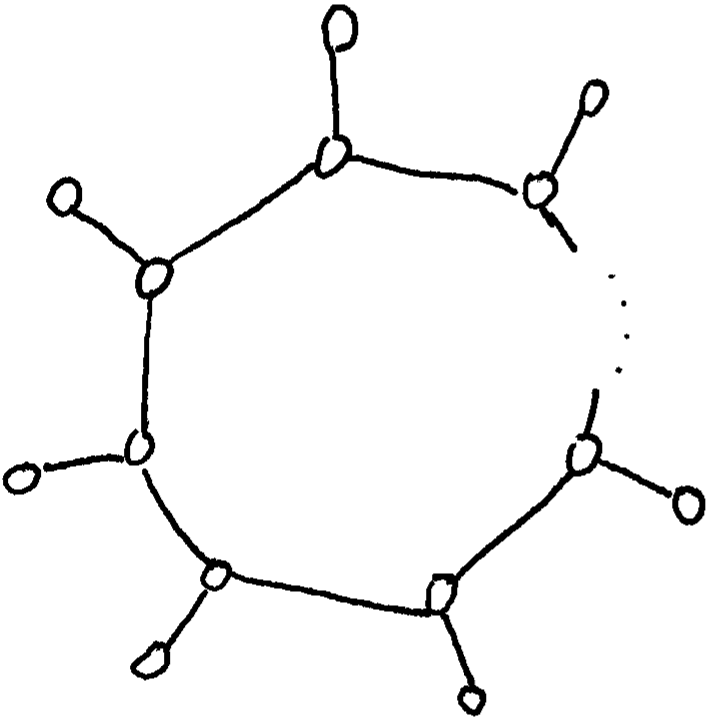
\includegraphics[width=0.4\textwidth]{graphics/modelltenta_graph_labellings.png}
    \caption{En graf för vilken vi skall räkna antalet sätt att etikettera den.}
\end{figure}

\section{Fråga 7 (5 poäng)} % del 3

En \emph{$k$-stjärna} i en graf $G$ består av en nod $v\in G$ tillsammans med $k$ stycken av dess grannar.

\begin{figure}
    \centering
    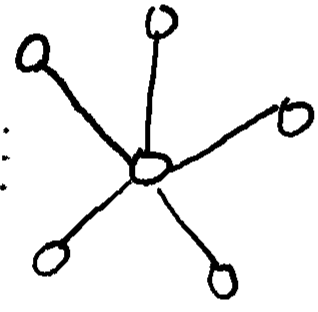
\includegraphics[width=0.35\textwidth]{graphics/modelltenta_star_graph.png}
    \caption{En $k$-stjärna, med en central nod och $k$ stycken noder runt omkring.}
\end{figure}

\noindent\textbf{Delfråga a:} \emph{(2p)}

Beräkna väntevärdet av antalet $k$-stjärnor i Erd\H{o}s-Renyi-grafen $G_{n,p}$.

\noindent\textbf{Delfråga b:} \emph{(3p)}

Använd vad du gjorde i förra delfrågan för att bevisa att, om $p_n = \frac{c}{n}$ för något $c > 0$, så gäller det att
$$\Prob{\max_{v \in G_{n,p_n}} d_v \geq \alpha n} \to 0\qquad\text{när }n\to\infty$$
för varje $\alpha > 0$.

\section{Fråga 8 (5 poäng)} % del 3

I ett av våra exempel på den probabilistiska metoden visade vi att varje graf $G = (V, E)$ på ett jämnt antal noder $n$, med $d_v \leq \frac{n}{2}$ för alla $v \in V$, har en uppdelning $V = A \coprod A^c$, med $\abs{A} = \frac{n}{2}$, sådan att
$$\abs{E(A, A^c)} \leq \frac{\abs{E}}{2}.$$

\noindent\textbf{Delfråga a:} \emph{(2p)}

Första delen av vårt bevis av detta var att skapa oss en matchning av noderna i grafen. Beskriv hur detta gick till.\sidenote[][]{Namnet på satsen vi använde här är \emph{Diracs sats}.}

\noindent\textbf{Delfråga b:} \emph{(3p)}

Använd matchningen vi skapade i förra delfrågan för att bevisa satsen.

\pagebreak

\section{Formelsamling}

\section{Den tolvfaldiga vägen}

\begin{fullwidth}
  \begin{tabularx}{\linewidth}{l|ccc}
    & Generellt $f$ & Injektivt $f$ & Surjektivt $f$\\
    \midrule
    Bägge särskiljbara & \specialcell{Ord ur $X$ av längd $n$\\ $x^n$} & \specialcell{Permutation ur $X$ av längd $n$\\ $\frac{x!}{(x-n)!}$} & \specialcell{Surjektion från $N$ till $X$\\$x!\stirlingPart{n}{x}$} \\
    Osärskiljbara objekt & \specialcell{Multi-delmängd av $X$\\ av storlek $n$\\$\binom{n + x - 1}{n}$} & \specialcell{Delmängd av $X$ av storlek $n$\\$\binom{x}{n}$} & \specialcell{Kompositioner av $n$\\av längd $x$\\$\binom{n - 1}{n - x}$} \\
    Osärskiljbara lådor & \specialcell{Mängdpartition av $N$\\ i $\leq x$ delar \\$\sum_{k=1}^{x} \stirlingPart{n}{k}$} & \specialcell{Mängdpartition av $N$\\ i $\leq x$ delar av storlek $1$\\$1$ om $n \leq x$, $0$ annars} & \specialcell{Mängdpartition av $N$\\i $x$ delar\\$\stirlingPart{n}{x}$} \\
    Bägge osärskiljbara & \specialcell{Heltalspartition av $n$ i $\leq x$ delar\\$p_x(n + x)$} & \specialcell{Sätt att skriva $n$ som\\summan av $\leq x$ ettor\\$1$ om $n \leq x$, $0$ annars} & \specialcell{Heltalspartitioner av $n$\\ i $x$ delar \\$p_x(n)$} 
  \end{tabularx}
\end{fullwidth}

\section{Räkneregler för genererande funktioner}

\begin{lemma}[Räkneregler för genererande funktioner]
  Antag att vi har en följd $\{a_k\}_{k=0}^\infty$, med genererande funktion $F_a$. Då gäller det att
    \begin{enumerate}
        \item För varje $j \geq 1$ är
        $$\sum_{k = j}^{\infty} a_k x^k = \left(\sum_{k=0}^{\infty}a_k x^k\right) - \left(\sum_{k=0}^{k=j-1} a_kx^k\right) = F_a(x) - \sum_{k=0}^{k=j-1} a_kx^k$$
        \item För alla $m \geq 0$, $l \geq -m$ gäller det att
        $$\sum_{k=m}^{\infty} a_k x^{k + l} = x^l\left(\sum_{k=m}^{\infty} a_k x^{k}\right) = x^l\left(F_a(x) - \sum_{k=0}^{m-1} a_k x^k\right)$$
        \item Det gäller att\sidenote[][]{Denna räkneregel kan förstås generealiseras till att högre potenser av $k$ motsvarar högre derivator -- och om vi istället delar med någon potens av $k$ får vi primitiva funktioner till den genererande funktionen.}
        $$\sum_{k=0}^{\infty} k a_k x^k = \frac{F_a'(x)}{x}.$$
    \end{enumerate}
\end{lemma}

\section{Vanliga genererande funktioner}

\begin{tabularx}{\linewidth}{cc}
  Följd & Genererande funktion\\
  \midrule
  $(1, 0, 0, \ldots)$ & $1$\\
  $(1,1,1,\ldots)$ & $\frac{1}{1-x}$\\
  $a_k = 1$ om $k \leq n$, $0$ annars & $\frac{1 - x^{n+1}}{1 - x}$\\
  Fixt $n$, $a_k = \binom{n}{k}$ & $(1+x)^n$\\
  Fixt $n$, $a_k = \binom{n+k-1}{k}$ & $\frac{1}{(1-x)^n}$\\
  \specialcell{Fibonaccitalen\\$f_0 = f_1 = 1$, $f_{k+1} = f_k + f_{k-1}$ för $k \geq 1$} & $\frac{1}{1 - x - x^2}$\\
  \specialcell{Indikatorfunktion för jämna talen\\$(1,0,1,0,1,0,\ldots)$} & $\frac{1}{1-x^2}$\\
  Catalantalen & $\frac{1 - \sqrt{1 - 4x}}{2x}$
\end{tabularx}

\begin{tabularx}{0.9\linewidth}{cc}
  Följd & Exponentiell genererande funktion\\
  \midrule
  $(1, 0, 0, \ldots)$ & $1$\\
  $(1, 1, 1, \ldots)$ & $e^x$\\
  $(0!, 1!, 2!, 3!, \ldots)$ & $\frac{1}{1-x}$\\
  Fixt $n$, $a_k = \frac{n!}{(n-k)!}$ & $(1 + x)^n$
\end{tabularx}

\section{Sannolikhetsteori}

\begin{lemma}
  Det gäller för alla händelser $A$ och $B$ att
  \begin{itemize}
      \item per definition är $\Prob{A} = \sum_{\omega \in A} \mu(\omega)$,
      \item så $\Prob{A^c} = 1 - \Prob{A}$,
      \item och om $A$ och $B$ har tomt snitt, $A\cap B = \emptyset$, så är $\Prob{A \cup B} = \Prob{A} + \Prob{B}$,
      \item och om de inte nödvändigtvis har tomt snitt har vi att
      $$\Prob{A \cup B} = \Prob{A} + \Prob{B} - \Prob{A \cap B}.$$
      \item $\Prob{A \cap B} = \Prob{A \given B}\Prob{B}$,
      \item och per definition är $A$ och $B$ oberoende precis när $\Prob{A \cap B} = \Prob{A}\Prob{B}$.
  \end{itemize}
\end{lemma}

\begin{lemma}
  Om $(\Omega, \mu)$ är något sannolikhetsrum, $A \subseteq \Omega$ någon händelse, och $X, Y: \Omega \to \R$ samt $Z: \Omega \to V$ är slumpvariabler som tar värden i $\R$ och i någon godtycklig mängd $V$, så gäller att:
  \begin{enumerate}
      \item $$\E{X} = \sum_{x \in X(\Omega)} x \Prob{X = x} = \sum_{\omega \in \Omega} X(\omega)\mu(\omega).$$
      \item För alla $a, b \in \R$ så är
      $$\E{aX + bY} = a\E{X} + b\E{Y}.$$
      Väntevärdet är alltså en linjär funktional.
      \item $$\Prob{A} = \E{\indSet{A}}.$$
      \item Om $X(\omega) \leq C$ för varje $\omega$, eller ekvivalent om $\Prob{X \leq C} = 1$, så är $\E{X} \leq C$.
      \item Om $\E{X} = C$ så finns det åtminstone ett $\omega$ sådant att $X(\omega) \geq C$.
      \item Om $Z$ är likformigt fördelad på $V$ så gäller det för varje delmängd $W \subseteq V$ att
      $$\Prob{Z \in W} = \frac{\abs{W}}{\abs{V}}.$$
  \end{enumerate}
\end{lemma}


\pagebreak

\section{Lösningsförslag}

På de frågor som är mer teori -- ge definitioner eller bevis ur kursen -- ges enbart sidhänvisningar till var i anteckningarna lösningen kan finnas. För övriga frågor ges lösningar.

\section{Fråga 1}

Höger led är uppenbarligen antalet sätt att välja ut $k$ personer ur en grupp av $m + w$ personer. Om vi tänker oss att vår grupp av personer består av $m$ män och $w$ kvinnor kan vi också tänka att vi först väljer hur många av personerna som skall vara män -- $j$ stycken, och $j$ kan vara mellan $0$ och $k$ -- och sedan väljer vi $j$ stycken män och $k-j$ stycken kvinnor. Detta är precis vad som pågår i vänster led.

\section{Fråga 2}

Den tolvfaldiga vägen diskuteras från sida tre till fem i föreläsning fyra.

\section{Fråga 3}

Detta är Exempel 5 på sida två i föreläsning fem. Alternativt kan man göra som i övning fyra på den föreläsningen.

\section{Fråga 4}

Detta är Teorem 11 i föreläsning fem, som vi bevisar på sida fem i den föreläsningen.

\section{Fråga 5}

Detta är Lemma 4 på sida två i föreläsning sju.

\section{Fråga 6}

\noindent\textbf{Delfråga a:}

Definitionerna som efterfrågas är spridda genom föreläsning åtta. Den term vi inte varit helt rigorösa med är ``oetiketterad graf'' -- den formella definitionen av detta vore egentligen ``isomorfiklass av grafer'', men eftersom vi inte använt sådan terminologi i kursen krävs den självklart inte på tentan.\sidenote[][]{Det här är egentligen samma sak som hur vi i den tolvfaldiga vägen inte definierat exakt vad vi menar med ``osärskiljbar'' -- där är också den rigorösa definitionen någonting med gruppverkan och symmetrier och så, vilket vi skippade.}

\noindent\textbf{Delfråga b:}

Grafen vi skall etikettera har uppenbarligen en rotationssymmetri. Vi kan se för varje nod om den är i den inre eller yttre ringen, och i vilken ordning dess grannar kommer, men vi kan inte referera till ``norra delen'' av cirkeln, eller något sådant.

Detta är alltså faktiskt en variant på vårt problem med att placera personer runt ett runt bord! Vi kan tänka oss det som att vi ska placera $2n$ personer runt ett runt bord med bara $n$ platser, så varje person måste få en annan som sitter i knät.

Så vi börjar med att välja vilka $n$ personer som skall få sitta på en stol, vilket vi kan göra på $\binom{2n}{n}$ sätt. Sedan placerar vi ut dessa runt det runda bordet -- vi vet från vår tidigare räkning i kursen att detta kan göras på $\frac{n!}{n} = (n-1)!$ sätt (varje av de $n!$ permutationerna kan roteras på $n$ sätt, så vi ``dividerar ut symmetrin''). Till slut väljer vi vems knä varje av de återstående personerna skall sitta i -- nu har vi inte kvar någon symmetri, eftersom personerna i stolarna nu fungerar som etiketter. Så vi kan göra detta på $n!$ sätt.

Så totalt har vi sett att svaret måste bli 
\begin{align*}
  \binom{2n}{n}(n-1)!n! &= \frac{(2n)!}{n!(2n-n)!}(n-1)!n!\\
  &= \frac{(2n)!}{n}.
\end{align*}

\section{Fråga 7}

\noindent\textbf{Delfråga a:}

En $k$-stjärna består av en central nod $v$ och en mängd $T\not\ni v$ av $k$ stycken noder som har en kant till $v$. Så låt $A_{v, T}$ vara händelsen att $v$ är centrum i en $k$-stjärna med $T$, alltså händelsen att alla kanter $\{v,w\}$ för $w\in T$ existerar.

Vi kan då räkna att
\begin{align*}
  \E{\#k-\text{stjärnor}} &= \E{\sum_{v\in V}\sum_{T \in \binom{V\setminus v}{k}} \ind{A_{v,T}}}\\
  &= \sum_{v\in V}\sum_{T \in \binom{V\setminus v}{k}} \E{\ind{A_{v,T}}}\\
  &= \sum_{v\in V}\sum_{T \in \binom{V\setminus v}{k}} \Prob{A_{v,T}}
\end{align*}
och eftersom $A_{v,T}$ bara är händelsen att en utpekad mängd av $k$ stycken kanter existerar, och kanter existerar oberoende av varandra med sannolikhet $p$, måste $\Prob{A_{v,T}} = p^k$, så
\begin{align*}
  \E{\#k-\text{stjärnor}} &= \sum_{v\in V}\sum_{T \in \binom{V\setminus v}{k}} p^k\\
  &= n\binom{n-1}{k}p^k.
\end{align*}

\noindent\textbf{Delfråga b:}

Låt oss börja med att observera att händelsen att
$$\max_v d_v \geq \alpha n$$
är precis händelsen att det finns en $\alpha n$-stjärna i grafen. Finns det en sådan stjärna har så klart dess centrum grad åtminstone $\alpha n$, och vice versa, finns det en nod av grad åtminstone $\alpha n$ kan vi ta den som centrum och $\alpha n$ av dess grannar som en stjärna.

Idén är att vi använder vad vi gjorde i förra räkningen, och ser att väntevärdet av antalet $\alpha n$-stjärnor går mot noll, och sedan använder Markovs olikhet för att få det uppgiften ber om.

Så vi kommer ihåg att $p = \frac{c}{n}$ och vad vi har sett i förra deluppgiften, och räknar
\begin{align*}
  \E{\#\alpha n-\text{stjärnor}} &= n \binom{n-1}{\alpha n}p^{\alpha n}\\
  &= n \frac{(n-1)(n-2)(n - \alpha n + 1)}{(\alpha n)!} \left(\frac{c}{n}\right)^{\alpha n}\\
  &\leq \frac{n^{\alpha n + 1}}{(\alpha n)!}\left(\frac{c}{n}\right)^{\alpha n}\\
  &= \frac{n c^{\alpha n}}{(\alpha n!)}
\end{align*}
och att detta uttryck går mot noll ser vi någorlunda enkelt -- täljaren är $n\cdot c \cdot c\cdot\ldots\cdot c$ och nämnaren är $\alpha n(\alpha n - 1)(\alpha n - 2)\ldots2\cdot1$, så den växer betydligt snabbare för varje fixt $\alpha$.

Markovs olikhet säger oss nu att
\begin{align*}
  \Prob{\max_{v \in G_{n,p_n}} d_v \geq \alpha n} &= \Prob{\#\alpha n-\text{stjärnor} > 1 - \epsilon}\\
  &\leq \frac{\E{\#\alpha n-\text{stjärnor}}}{1 - \epsilon}\\
  &< \E{\#\alpha n-\text{stjärnor}} \to 0
\end{align*}
vilket är vad vi ville visa.

\section{Fråga 8}

Beviset av detta är Proposition 4, på sidan två av föreläsning 11.

%\bibliography{references}
%\bibliographystyle{plainnat}

\end{document}
